\chapter{Literature Review}
To determine the most optimal design and implementation tool, I conducted a comprehensive evaluation of the various cloud technologies. This involved exploring the capabilities of each cloud technology, and diving into the supporting documentation. By understanding the objectives, strengths, and weaknesses of each of the different technologies, I was able to narrow down on the problem that I was trying to solve, and select the best tools that will align with the requirements of the project.

\section{Infrastructure as Code (IaC)}
According to AWS, “Infrastructure as Code (IaC) is the ability to provision and support your computing infrastructure using code instead of manual processes and settings.”. In the typical software development life cycle, when it gets to deploying applications, developers have to regularly set up, update, and maintain infrastructure in order to develop, test, and deploy applications \cite{aws-iac}. 

With more and more applications coming up, and companies focusing on high velocity, it has become increasingly important for these manual tasks like infrastructure provisioning to be automated. Furthermore, manual infrastructure provisioning is also more error prone, especially when managing applications at scale (AWS, n.d.). As such, more and more IaC tools have come up, so that infrastructure can be provisioned reliably, quickly, and unambiguously to support our applications in the cloud. Next, we will discuss some of the common IaC tools, their uses cases, strengths as well as pitfalls. 



\subsection{Terraform}
Perhaps one of the most popular IaC tools is Terraform. Terraform is an open-source IaC tool created by HashiCorp, which allows users to define and provision infrastructure declaratively. With Terraform, one can specify infrastructure resource in human-readable configuration files that can be reused, distributed, and modified \cite{cloud-2023}. 

\textbf{\textit{Benefits}}
\begin{enumerate}
\vspace{-1em}
    \item \textbf{Flexibility and Scalability:} Terraform integrates with over 1700 service providers governing different types of resources and services \cite{cloud-2023}, which means that developers can automate the deployment and management of a wide variety of resources ranging from compute instances to storage solutions.
    \item \textbf{Cloud Agnostic:} Terraform is cloud agnostic, meaning that a single configuration can manage multiple providers and handle cross-cloud dependencies.
    \item \textbf{Open Source:} Terraform is open source and free to use.
    \item \textbf{State Management:} Terraform manages its own state, meaning that cloud resources created and destroyed are all kept track of in a Terraform state file. This eliminates the worry of dangling or failed-to-provision resources.
\end{enumerate}

\textbf{\textit{How Terraform Works}}
\vspace{-1em}
\begin{enumerate}
    \item \textbf{Providers:} At a high level, Terraform creates resources based on the targets exposed application programming interfaces (APIs). Communication with these APIs happens through providers, which are plugins that interact with various platforms and manage their resources. These providers can be seen as a logical abstraction of an upstream API. Today, Terraform supports over 1800 providers, including major cloud providers such as AWS and GCP, as well as providers for Docker, Kubernetes, and more \cite{cvitkovic-2022}. Providers are normally defined in a top-level \texttt{terraform.tf} file as shown below:
    \begin{verbatim}
terraform {
  required_providers {
    aws = {
      source  = "hashicorp/aws"
      version = "~> 5.47.0"
    }
  }
  required_version = "~> 1.3"
}
    \end{verbatim}
    \item \textbf{terraform plan:} This command creates an execution plan, which generates a preview of the changes that Terraform plans to make to your infrastructure \cite{hashicorp}. By default, the following steps are taken:
    \begin{enumerate}
        \item Reads the current state of any already-existing remote objects to ensure that the Terraform state is up-to-date.
        \item Compares the current configuration to the prior state and generates a difference between the current and prior state.
        \item Proposes a set of changes that, if applied, will make the remote objects match the configuration.
    \end{enumerate}
    \item \textbf{terraform apply:} This command executes the actions proposed in a Terraform plan \cite{hashicorp}. By default, the following steps are taken:
    \begin{enumerate}
        \item All the steps as detailed in the above section on \texttt{terraform plan}.
        \item Prompt for plan approval. For auto-approval, the flag \texttt{--auto-approve} can also be passed to the \texttt{terraform apply} command.
        \item Undertakes the actions as indicated in the plan to modify existing cloud infrastructure to meet the desired current state.
        \item Modifies the state file to match the current state.
    \end{enumerate}
    \item \textbf{terraform destroy:} This command is used as a way to destroy all remote objects managed by a particular Terraform configuration \cite{hashicorp}.
    \item \textbf{The Terraform State File:} To make all of the above possible, Terraform needs to maintain some kind of state, so that it is aware of the current state of resources on the cloud. This is done through the \texttt{terraform.tfstate} file, which is automatically generated/modified on every Terraform command that mutates state. For local development of Terraform, the \texttt{terraform.tfstate} file is generated locally. For production and other higher environments, it is standard practice for the \texttt{terraform.tfstate} file to be stored in the cloud, such as an S3 bucket, with DynamoDB for locking, to ensure effective version control \cite{deepeshjaiswal-2024}.
\end{enumerate}

\begin{figure}[h!]
    \centering
    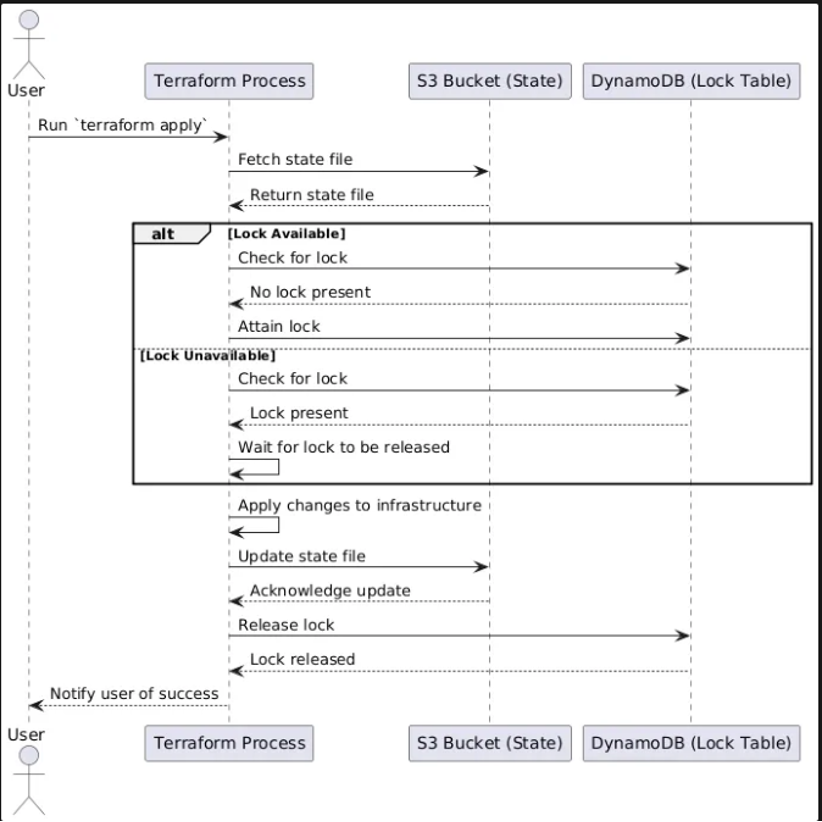
\includegraphics[width=0.8\textwidth]{fig/typical-tf-backend.png}
    \caption{Sequence Diagram for Terraform Backend}
    \label{fig:tf-backend}
\end{figure}

The above diagram shows the typical workflow in handling terraform state files. In summary, state files are usually saved to some storage such as an S3 bucket. Access to these state files are then synchronized via a lock, which is commonly implemented in DynamoDB \cite{deepeshjaiswal-2024}. This allows race-free interaction with the provisioned infrastructure.


\subsection{AWS CloudFormation}
AWS CloudFormation is an IaC tools that allows one to manage infrastructure and automate any deployments using code \cite{aws-cloudformation}. CloudFormation is also done declaratively, and written in familiar languages such as YAML or JSON. This makes managing, scaling, and automating AWS resources fast and straightforward. However, the greatest downside is that CloudFormation is part of the AWS stack, and is not cloud agnostic. This means that developers are reliant on the AWS cloud should they choose to use AWS CloudFormation. 

\subsection{OpenTofu}
OpenTofu is yet another open-source IaC tool designed to help with the provisioning and management of infrastructure \cite{dinu-2024}. It holds many similarities to Terraform as discussed above, but has an added feature of allowing for state encryption. There are also some differences in their licensing which will not be discussed here. 

\subsection{Ansible}
Ansible is an open-source automation tool used for configuration management, application deployment, and task automation. Unlike Terraform and CloudFormation, which are declarative, Ansible uses an imperative approach to define the desired state of the infrastructure. The greatest upside of Ansible is that it is agentless, meaning it does not require any software to be installed on the target machines.

\section{IaC Orchestration and Frameworks}
IaC orchestration is used to enforce good programming practices, improving code readability and quality. This provides additional structure, automation, and improves maintainability for complex infrastructure. These tools provide a significant advantage over pure Terraform by improving code readability, promoting consistency across projects, and enabling faster collaboration and development in multi-environment setups. 

Several IaC orchestration tools have also been built on top of terraform, such as terragrunt and terraspace. While an IaC orchestration tool will not be used in the implementation due to the main aim of keeping cloudkube portable and easily distributable, it is important to note how these tools fit into the whole cloud ecosystem.

\subsection{Terragrunt}
Terragrunt is a thin wrapper that is written on top of terraform, that provides some tooling and opinions \cite{nguyen-2020}. Terragrunt also provides a way to keep your code DRY by using the generate helper method. Terragrunt also helps in the automated creation of backends, which can be a chore if using raw terraform. Lastly, terragrunt allows for the injection of CLI hooks, allowing the utility to execute custom actions before or after terraform commands

\subsection{Terraspace}
Terraspace is a framework, which allows developer to dynamically generate terraform project in a centralized manner \cite{nguyen-no-date}. It is highly opinionated, and strongly enforces modularity and DRYness through stacks. On top of all the benefits offered by terragrunt, terraspace also allows the easy segregation of development and high-level environments through terraspace layering, which allows for the usage of the same code to deploy and create multiple environments. 

\section{Container and Container Orchestration}
Containerisation has become the standard practice of the industry today. Allowing for quicker software development cycles, together with more efficient CI/CD practices and portability, containerisation provides us a powerful, and agile way to manage our applications \cite{rgs-2023}. Along with the growing complexity of distributed systems, container orchestration software such as Kubernetes are also used to automate deployment, handle scalability and fault tolerance, as well as efficient resource utilization.
This chapter will discuss some of the common container and container orchestration software, which are pertinent to this project given that most SpeechLab applications have been containerised for the cloud

\subsection{Docker}
Docker is a containerisation software which aids in development, shipping, and deployment. Docker enables the separation of application from infrastructure so that software can be delivered quickly and reliably \cite{docker-docs-2024}. With docker, code, as well as version-locked dependencies are baked into a container image. This means that anyone building from this image on any machine in the world, regardless of architecture, will build the same thing, and run the same application. This creates reproducible environments of an application based on a single Docker Image. 

\subsection{Kubernetes}
Kubernetes is an open-source container orchestration software that helps to automate deployment, scale, and manage containerised applications. Kubernetes provides a framework to run distributed systems resiliently, taking care of scaling and failover of the application \cite{kubernetes-docs}. 

\textbf{\textit{Key Features of Kuberentes}}
\begin{enumerate}
    \vspace{-1em}
        \item \textbf{Self-healing: } Kubernetes restarts, replaces, or kills containers that are unhealthy, and doesn’t advertise these containers to clients until they are ready to serve.
        \item \textbf{Storage Orchestration:} Kubernetes allows the automatic mounting of a storage system of the developers choice.
        \item \textbf{Horizontal Scaling: } Kubernetes can scale up or down an application with a simple command, UI, or automatically based on user-defined parameters.
        \item \textbf{Service Discovery and Load Balancing: } Kubernetes can expose a container using the DNS name of the container, or using its own IP address. Kubernetes can also load balance and distribute network traffic to ensure deployment stability. 
\end{enumerate}

\textbf{\textit{Kubernetes Architecture}}
\begin{figure}[h!]
    \centering
    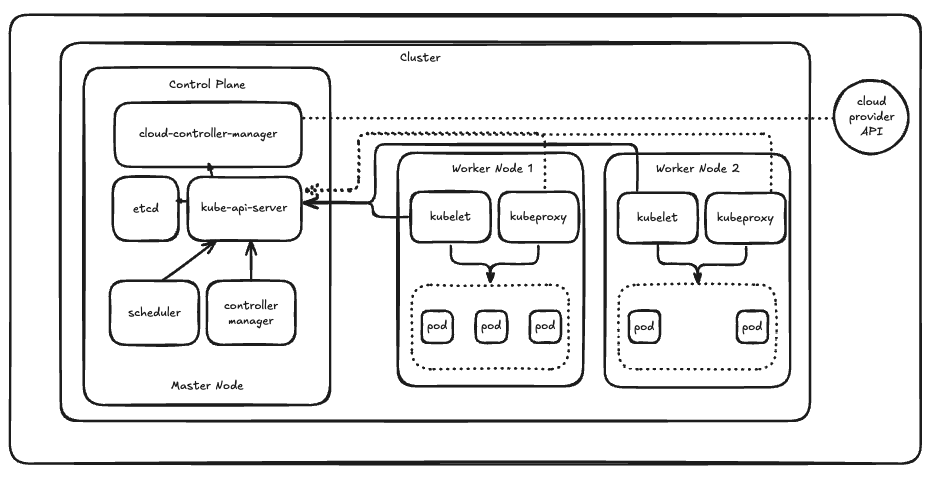
\includegraphics[width=1\textwidth]{fig/kubernetes-cluster-architecture.png}
    \caption{Typical Kubernetes Architecture}
    \label{fig:k8s-architecture}
\end{figure}

A Kubernetes cluster typically comprises the Control Plane as well as multiple Worker Nodes. Each of these nodes hold different responsibilities, which are detailed below.


\begin{enumerate}
    \vspace{-1em}
        \item \textbf{Master Node}
        \begin{enumerate}
            \item The Kubernetes master node, also known as the control plane, is the controller of the whole system. This is where all operational decisions are made, including scheduling, balancing, and responding to events.  
            \item \textit{kube-api-server:} The Kubernetes API Server is the main module within the master node which receives all REST requests for modifications, thereby serving as the frontend to the cluster \cite{bindlish-2021}. It acts as an interface for interaction with the cluster. 
            \item \textit{kube-controller-manager:} The kube-controller-manager runs a distict number of daemon processes, which help to regulate the shared state of the cluster, as well as perform routine tasks. When changes in configurations occur, the kcm is responsible for spotting the change and working toward the new desired state \cite{bindlish-2021}. 
            \item \textit{Kube-scheduler:}  The Kubernetes scheduler helps to schedule the pods on the various nodes based on resource utilization \cite{bindlish-2021}. The kube-scheduler is aware of all the resources available, and is responsible for allocating pods to nodes in an efficient manner to avoid resource exhaustion. Should no resources be available, the kube-scheduler puts pods in a pending state until resources are available again.
            \item \textit{etcd:} The etcd is a highly available, distributed key-value store that is use by Kubernetes to store cluster configuration data and state information. It keeps track of all cluster components such as nodes, pods, deployments and network configurations. 
        \end{enumerate}
        \item \textbf{Worker Nodes}
        \begin{enumerate}
            \item The Kubernetes worker node, is a worker machine in the Kubernetes cluster. There can be multiple worker nodes in a Kubernetes cluster. Each node is responsible for running pods, and is managed by the master node. These worker nodes are the workhorses of the Kubernetes cluster, and all application execution logic is carried out in these worker nodes. 
            \item \textit{kubelet:} The kubelet is the main service on a node, which regularly takes in pod specifications through the kube-api-server. The Kubelet is responsible for ensuring that pods and containers are healthy, and running in the desired state \cite{bindlish-2021}. The Kubelet is also responsible for health checks. 
            \item \textit{kube-proxy}: The kube-proxy is a service that runs on each worker node, that deals with networking. It is responsible for exposing services to the external world, or to the rest of the cluster. It performs request forwarding to the correct pods across various isolated networks in a cluster \cite{bindlish-2021}.
            \item \textit{Container runtime:} The container runtime is responsible for pulling images from a container image registry (i.e. Dockerhub, Amazon AWS ECR), and starting and stopping containers. The most common plugin used for this is Docker \cite{bindlish-2021}.
        \end{enumerate}
        \item \textbf{Pods}
        \begin{enumerate}
            \item A pod is the smallest unit that can be scheduled in Kubernetes \cite{bindlish-2021}. Pods help in scalability through replication. In the case of errors or failed health checks, Kubernetes also creates new pods, and destroys unhealthy ones. A single pod can contain multiple containers, and these containers share an IP address and port space, and are able to communicate internally via localhost.
        \end{enumerate}
\end{enumerate}

\textbf{\textit{Networking in Kubernetes}}

Another concept relevant to the development of \texttt{cloudkube} is networking in Kubernetes. The following section will two main networking concepts in Kubernetes, which will become relevant to our implementation in Chapter 4.
\begin{enumerate}
\item \textbf{Service: }A service in Kubernetes is a logical abstraction that provides stable networking for a group of pods running in a cluster. It enables communication between Pods, and ensures consistent access to applications, even if individual pods are created or deleted. These services can act as load balancers to distribute traffic across multiple pods. Pods with type \texttt{ClusterIP} work to expose services internally whthin the cluster. Pods with type \texttt{NodePort} exposes a service on a static port on each node, and pods with type \texttt{LoadBalancer} provisions an external load balancer in the cloud to publicly expose services. 
\item \textbf{Ingress: }A Kubernetes ingress object is an API object that manages external access to services in a cluster, typically through HTTP/HTTPS. The Ingress object allows us to map traffic to different backends based on rules defined via the Kubernetes API. 
\item \textbf{Ingress Controller: }In order for an Ingress to work in the cluster, there must be an ingress controller running. Ingress controllers are not started automatically with a cluster, and requires a one to be specified and provisioned for ingress resources to work. 
\end{enumerate}

\textbf{\textit{Storage in Kubernetes}}

Lastly, this section will detail how Kubernetes handles ephemeral and persistent storage. Similarly, this becomes relevant to our implementation as detailed in Chapter 4.
\begin{enumerate}
    \item \textbf{Volumes: } Volumes in Kubernetes provide a way for containers in a pod to access and share data via the filesystem. This can be used for data sharing between two different containers in the same pod, or even between two different pods. There are two broad categories of volumes. Ephemeral volume types have the lifetime of a pod, and follow the lifecycle of a pod, while persistent volumes exist beyond the lifetime of a pod.  
    \item \textbf{Persistent Volumes (PV): } A persistent volume is a piece of storage in the cluster that has been provisioned by the developer. The data in the PV remains even after pods are destroyed or recreated. 
    \item \textbf{Persistent Volume Claims (PVC): } A Persistent Volume Claim is a request for storage by a user. PVCs consume PV resources, and have defined access modes, such as ReadWriteOnce, ReadOnlyMany, ReadWriteMany, or ReadWriteOncePod. 
\end{enumerate}

\section{Infrastructure and Cloud}
This chapter details some of the key cloud infrastructure that is provisioned in order to host speech applications. For a proof of concept, and due to limited access to various clouds, everything in this paper is hosted on the AWS cloud. However, it should be noted that many of these concepts (such as VPC, subnets, load balancers etc.) are similar in other clouds, and \texttt{cloudkube} is extendable to other cloud providers as well. Each subsection will discuss the main uses of each of these components, and briefly detail the corresponding names of these components in AWS, Microsoft Azure Cloud, as well as Google Cloud Provider.

\begin{figure}[h!]
    \centering
    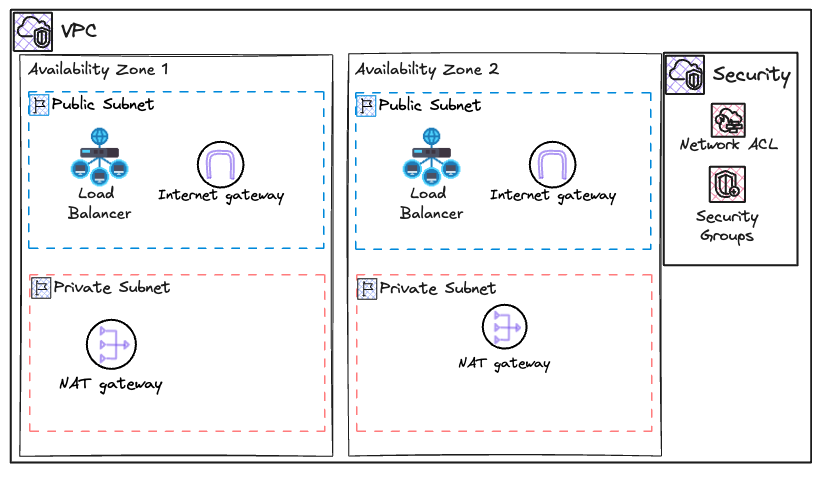
\includegraphics[width=\textwidth]{fig/vpc-subnets.png}
    \caption{Relationship between VPC, Subnets, and other basic cloud componenets}
    \label{fig:vpc-subnets}
\end{figure}


\subsection{Virtual Private Cloud (VPC)}
A virtual private cloud allows the creation of logically isolated sections of the cloud where different resources can be launched in a user-defined virtual network. Developers have full control over the virtual networking environment, including the selection of IP address ranges, creation of subnets, as well as configuration of route tables and network gateways. There will be mentions of some VPC related terminology in the following chapters, all of which are defined here.

\begin{itemize}
    \vspace{-1em}
    \item \textbf{Subnets: } Subnets allow the division of the VPC into different IP address ranges. They can be public or private.
    \item \textbf{Route Tables: } Route Tables allow the control of routing of traffic within the network. This helps in directing traffic between subnets, or between different VPCs.
    \item \textbf{Internet Gateway (IGW): } The Internet Gateway can be attached to a VPC to allow communication between resources in the VPC and the internet.
    \item \textbf{NAT Gateway: } The Network Address Translation (NAT) Gateway enables instances in a private subnet to connect to the internet or other cloud services while preventing the internet from initiating a connection with those instances.
    \item \textbf{Security Groups / Network Access Control Lists (ACLs): } These are virtual firewalls that control ingress and egress traffic at the instance and subnet levels, providing granular security controls.
\end{itemize}

\textbf{Cloud Provider VPCs}
\begin{itemize}
    \vspace{-1em}
\item AWS Cloud: AWS Virtual Private Cloud
\item GCP: Virtual Private Cloud Network
\item Microsoft Azure: Virtual Networks
\end{itemize}

\subsection{Subnets}
A subnet is a range of IP addresses in a VPC. Subnets allow us to segment the network inside the VPC to group resources and control their access to each other and to the outside world. A subnet can be thought of as a sub-network within a VPC, where resources like EC2 instances can reside.  

\textbf{Key Features of Subnets}
\begin{enumerate}
    \vspace{-1em}
\item Public and Private Subnets
    \begin{itemize}
    \item Public Subnets are subnets with a route to an IGW. Instances within this subnet can directly communicate with the internet, provided that they have a public IP address or an Elastic IP.
    \item Private subnets are subnets which do not have a route to an IGW. Instances in a private subnet cannot communicate with the internet directly. They can only access the internet via a NAT Gateway, or NAT instances in a public subnet.
    \end{itemize}
\item CIDR Blocks (Classless Interdomain Routing)
 \begin{itemize}
    \item Each subnet is associated with a CIDR block that defines its IP address range. CIDR blocks of subnets are always within (longer prefix mask) the CIDR block of the VPC.
\end{itemize}
\item Availability Zones (AZ)
\begin{itemize}
    \item Subnets are created within a specific AZ in a region. Resources within a subnet are guaranteed to be located within the same AZ.
    \item Distribution of subnets across multiple AZs help to increase availability and fault tolerance. 
\end{itemize}
\item NACLs
\begin{itemize}
    \item Subnets are protected using NACLs, which are stateless firewalls that operate at the subnet level. They control ingress and egress traffic to and from the subnets based on user-defined rules.  
    
\end{itemize}
\end{enumerate}

\subsection{Virtual Machines}
Kubernetes applications that run in the cloud require compute to be done on virtual machines. Virtual machines are web services offered by cloud providers which allow users to run virtual servers in the cloud. The virtual machines are normally configurable in terms of the choice of processor, storage, networking as well as operating systems. 

\textbf{Cloud Provider Virtual Machines}
\begin{itemize}
    \vspace{-1em}
\item AWS Cloud: AWS Elastic Compute Cloud (EC2)
\item GCP: Google Compute Engine (GCE)
\item Microsoft Azure: Azure Virtual Machine (VM)
\end{itemize}

Pertinent to this paper, EC2 instances will be provisioned as nodes in the Kubernetes cluster. The Kubernetes pods are then ultimately run on these nodes.  

\subsection{Security Groups}
Security groups are virtual firewalls that control inbound and outbound traffic to and from resources. Security groups are stateful, meaning that if you allow an incoming request from a particular IP address and port, the response is automatically allowed without needing a separate outbound rule. Some cloud providers such as Azure also draw a distinction between security groups which operate at the application layer (operating on compute instances and services), as well as the network layer (operating on ingress and egress IP addresses and protocols).

\subsection{Elastic Network Interfaces (ENI)}
An ENI is a logical networking component in a VPC that represents a virtual network card. These ENIs are attached to instances launched in the same AZ. Every VM instance has a primary ENI attached by default, providing the instance with networking capabilities. These ENIs have multiple use cases. Pertinent to this paper, the ENIs are used to facilitate communication between the Kubernetes control plane and worker nodes within the cluster.  

\subsection {Instance Templates}

Instance Templates allow users to define the configuration for launch VM instances in a more flexible and reusable way. They allow the specification of instance parameters such as instance type, key pair, security groups and more. These templates can then be used by Auto Scaling Groups, Spot Fleets, and other services to provision VM instances according to the configurations specified. 

\textbf{Cloud Provider Instance Templates}
\begin{itemize}
    \vspace{-1em}
\item AWS Cloud: AWS Launch Template
\item GCP: Instance Templates
\end{itemize}

Appendix \ref{appendix:cloudformation-eks-vpc-yaml} shows an example AWS Launch Template to provision a VPC for use with Kubernetes.

\subsection{Managed Kubernetes Service}

Managed Kubernetes Services are services offered by cloud providers which can be used to run Kubernetes without needing to install, operate, and maintain your own Kubernetes control plane or nodes. The managed Kubernetes service is able to automatically scale control plane instances based on load, detect and replace unhealthy control plane instances, and provide automated version updates and patching for them. These managed service also often offer easy integrability with other cloud services such as file systems for persistent volume storage, and load balancing for load distribution.

\textbf{Cloud Provider Managed Kubernetes Service}
\begin{itemize}
    \vspace{-1em}
\item AWS Cloud: Elastic Kubernetes Service (EKS)
\item GCP: Google Kubernetes Engine (GKE)
\item Microsoft Azure: Azure Kubernetes Service (AKS)
\end{itemize}

\subsection{File Systems}
File systems provide a simple, serverless, set-and-forget elastic file system for use with cloud resources or on premise infrastructure. They are built to scale on demand to petabytes without disrupting applications, growing and shrinking automatically as files are added or removed, thereby eliminating the need to provision and manage capacity to accommodate growth. 

\textbf{Cloud Provider File Systems}
\begin{itemize}
    \vspace{-1em}
\item AWS Cloud: Elastic File System (EFS)
\item GCP: Cloud Filestore
\item Microsoft Azure: Fileshare
\end{itemize}

\subsection{Scaling Groups}
Often times, it is important for compute instances to automatically scale with load. Scaling groups are a collection of compute instances treated as a logical grouping. Its main purpose and objective is to provide for automatic scaling and management. This allows the user to maintain the number of instances in a scaling group. The scaling group starts by launching enough instances to meet its desired capacity. It then maintains this number of instances by conducting periodic health checks on instances in the group. If an instance becomes unhealthy, the scaling group then terminates the instance and launches another instance to replace it.  

\textbf{Cloud Provider Scaling Groups}
\begin{itemize}
    \vspace{-1em}
\item AWS Cloud: Auto Scaling Groups (ASG)
\item GCP: Managed Instance Groups (MIG)
\item Microsoft Azure: Azure Virtual Machine Scale Sets (VMSS)
\end{itemize}

\subsection{minikube}
minikube is a way for one to quickly set up a local Kubernetes cluster. It is compatible with macOS, Linux and Windows. The main goal of minikube is to help application developers do quick testing of their Kubernetes deployments locally, as well as a tool used for learning by new Kubernetes users \cite{minikube-docs}. By default, minikube creates a one-node cluster locally, and supports addons such as ingress controllers. As we will see in the following chapter, cloudkube functionality closely mirrors that of minikube, supporting the objective of cloudkube which is to provide a quick and easy testing environment for Kubernetes developers in the cloud.

\section{Past FYPs}
Past FYPs have worked on the deployment of Speech Recognition Systems to on-prem bare metal resources \cite{yap-2023}, as well as the AWS Cloud.
Benjamin Chen and Poh Kai Kiat worked to set up the CI/CD pipelines for versioning of the ASR system using Jenkins, ArgoCD and Gitlab \cite{chen-2021} \cite{poh-2022}. 
Tjandy Putra's work helped to bolster security measures through Kyverno and Falco \cite{putra-2023}. Ma Xiao helped to set up the 
barebones deployment of the Speech Recognition System on the AWS cloud via the AWS console \cite{ma-2021}. Lastly, Song Yu and Lee Kai Shern
introduced terraform to help handle the infrastructure provisioning \cite{song-yu-2023} \cite{lee-2022}. 

These FYPs have done great work in deploying the ASR application. However, the deployment process is inherently tightly coupled with the 
ASR application, and changes to source code or structure of the application requires significant recalibration of cloud resources. As such, this 
FYP aims abstract away the process of infrastructure provisioning, and provide an automated tool for a Kubernetes cluster to be spun up easily in the cloud. 
As a stretch goal, this FYP also aims to be extendable to other SpeechLab applications. This will allow SpeechLab developers to focus on core application logic, and 
simply call the \texttt{cloudkube} API to spin up a Kuberenetes cluster, and deploy their applications. 